\documentclass{beamer}


\setbeamerfont{footnote}{size=\tiny}
%\AtBeginSection[]
%{
%  \begin{frame}<beamer>
%%    \frametitle{Outline for Section \thesection}
%    \frametitle{Outline}
%    \tableofcontents[currentsection]
%  \end{frame}
%}

\newcommand{\OutlineRedux}
{
  \begin{frame}<beamer>
%    \frametitle{Outline for Section \thesection}
    \frametitle{Outline}
    \tableofcontents[currentsection]
  \end{frame}
}



\usepackage{bbm}
\usepackage{algorithm}
\usepackage{algpseudocodex}
\usepackage{caption}
%\usepackage{mathtools}
\usepackage{tikz}
\usetikzlibrary{positioning, arrows.meta}
\usetikzlibrary{decorations.pathreplacing,calligraphy}
\usepackage{hyperref}
\hypersetup{colorlinks=true, linkcolor=black, urlcolor=blue, citecolor=red}

\usetheme{CambridgeUS}
\setbeamercolor{title}{bg=red!65!black,fg=white}
% Include/Remove page numbering
\setbeamertemplate{page number in head/foot}{}


\setbeamertemplate{sidebar right}
{
  \vfill%
  \llap{\insertlogo\hskip0.1cm}%
  \vskip2pt%
  \llap{\href{http://domdisanto.github.io}{Downloadable Slides}\hskip0.2cm}% NEW
  \vskip3pt% NEW
  \llap{\usebeamertemplate***{navigation symbols}\hskip0.1cm}%
  \vskip2pt%
}



% Bibliography Options 
\usepackage[url=false, doi=false, maxcitenames=1, isbn=false]{biblatex}
\addbibresource{GNN_Presentation.bib}

\title{Graphical Neural Networks}
%\subtitle{}
\author{Dominic DiSanto}
\institute[]{Department of Biostatistics, Harvard University}
\date{\today}


% Custom commands 
\newcommand{\nhood}{\mathcal{N}}
\newcommand{\Graph}{\mathcal{G}}
\newcommand{\NodeSet}{V}
\newcommand{\NumNodes}{N}
\newcommand{\node}{v}
\newcommand{\nrepresent}{h}
\newcommand{\NodeRepMat}{\mathbf{H}}
\newcommand{\EdgeSet}{E}
\newcommand{\edge}{e}
\newcommand{\DegMat}{\mathbf{D}}
\newcommand{\iter}{\kappa}
\newcommand{\Iter}{K}
\newcommand{\AdjMat}{\mathbf{A}}
\newcommand{\LapMat}{\mathbf{L}}
\newcommand{\LapMatNorm}{\widetilde{\mathbf{L}}}
\newcommand{\ReLu}{\text{ReLu}}
\newcommand{\Ind}{\mathbbm{1}}
\newcommand{\Identity}{\mathbf{I}}
\newcommand{\Agg}{\text{Aggregate}}
\newcommand{\Msg}{\text{Message}}
\newcommand{\Loss}{\mathcal{L}}
\newcommand{\relation}{r}
%\newcommand{\relate}{r}
\newcommand{\RelationSet}{\mathcal{T}_R}
%%%%%%%%%%%%%%%%%%%%%%%%
    % START %%%%%%%%%%%%
%%%%%%%%%%%%%%%%%%%%%%%%
\begin{document}


\begin{frame}
\maketitle
\end{frame}

\begin{frame}{Outline}
\tableofcontents 
\end{frame}


\section{Set-Up and Motivation}

\begin{frame}{Goals}
    \begin{itemize}\setlength\itemsep{8mm}
        \item Briefly motivate and introduce Graphical Neural Networks (GNN)
        \item Describe recent reviews and applications 
        \begin{itemize}
            \item Drug Discovery 
            \item Multimodal Biomedical Data 
            \item Knowledge Graph Integrated GNN's \& TxGNN
        \end{itemize}
    \end{itemize}
\end{frame}

\begin{frame}{Knowledge Graph Data}
    \begin{figure}
        \centering 
        \includegraphics{txGNN_KG.png}
        \caption{Fig 1A from Huang (2023) \cite{huang_zero-shot_2023}}
    \end{figure}
\end{frame}
\begin{frame}{Multi-modal Biomedical Data}
    \begin{figure}
        \centering 
        \includegraphics[scale=0.2]{MultimodalPreview.png}
    \end{figure}
    Image courtesy of partial figure from McDermott et al. {\it Structure-inducing pre-training} \cite{mcdermott_structure-inducing_2023}
\end{frame}


\begin{frame}{Molecular/Biochemical }
    \begin{figure}
        \centering
        \includegraphics[scale=0.3]{Caffeine_Graph.png}
    \end{figure}
    Image courtesy of \url{https://distill.pub/2021/gnn-intro/} \cite{sanchez-lengeling_gentle_2021}
\end{frame}

\begin{frame}{Protein Representation }
    \begin{figure}
        \centering
        \includegraphics[scale=0.45]{Zhang_Protein3D.png}
    \end{figure}
    Fig 2. of Zhang (2023) {\it Geometric Deep Learning for Structure-Based Drug Design: A Survey} \cite{zhang_systematic_2023}
\end{frame}

\begin{frame}{Motivation}
    \begin{itemize}
        \item Want to utilize the input structure of the graph
        \begin{itemize}
            \item Respect/Maintain
            \item Update/Estimate
        \end{itemize} 
        \item "Flattening" graphical data for DNN, CNN, etc. omits useful topology from our data 
        \item Early methods attempting to retain topological info included recursive neural networks and random walk models, which GNN methodology extended \cite{scarselli_graph_2009} 
    \end{itemize}
\end{frame}



\begin{frame}{Notation/Set-Up}
    \begin{columns}[T] % align columns at the top
        \begin{column}{.7\textwidth}
            \begin{itemize}%{.5\textwidth}
                \setlength\itemsep{8mm}
%                \item Consider random vector $X \sim F(\boldsymbol\mu, \Sigma)$ and precision matrix $\Theta \equiv \Sigma^{-1}$
                \item Consider the graph $\Graph = (\NodeSet, \EdgeSet), \EdgeSet \subseteq \NodeSet \times \NodeSet$, where any node $\node$ has a related "feature vector" $x_\node \in \mathbb{R}^d$
                \begin{itemize}
                    \item Let $\NumNodes = |V|$
                \end{itemize}
                \item Let $\nhood_s(\node)$ represent the $s$-hop neighborhood of any node $\node$ (and implicitly $\nhood(\node) \equiv \nhood_1(\node)$)
                \item Can construct adjacency matrix $\AdjMat \in \mathbb{R}^{\NumNodes \times \NumNodes}$ to capture structure of edge set $\EdgeSet$ 
                \begin{itemize} 
                    \item $\AdjMat_{ij}=w_{ij}\Ind\{(i,j) \in \EdgeSet\}$ for scalar weight $w_{ij} \in \mathbb{R}$
                \end{itemize}
            \end{itemize}
        \end{column}
        \begin{column}{.3\textwidth}
            %\begin{figure}
                \centering
            \scalebox{0.9}{
                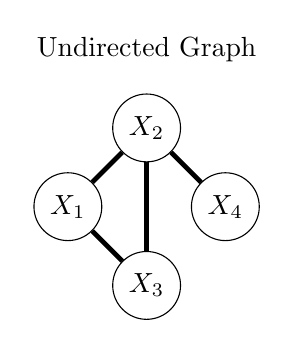
\begin{tikzpicture}
                \node[circle, draw] (A) at (0,0) {$X_1$};
                \node[circle, draw] (B) at (1,1) {$X_2$};
                \node[circle, draw] (C) at (1,-1) {$X_3$};
                \node[circle, draw] (D) at (2,0) {$X_4$};
                \node[] (capt) at (1, 2) {Undirected Graph};
                \draw[line width=0.6mm] (A) -- (B);
                \draw[line width=0.6mm] (A) -- (C);
                \draw[line width=0.6mm] (B) -- (D);
                \draw[line width=0.6mm] (C) -- (B);
            \end{tikzpicture}
            }
            %\caption{Undirected Graph}
            %\end{figure}
            \\ \vspace{3mm}
            \scalebox{0.9}{
            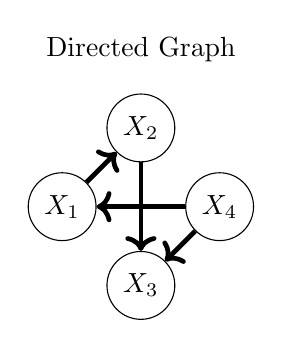
\begin{tikzpicture}%[opacity=0.2]
                \node[circle, draw] (A) at (0,0) {$X_1$};
                \node[circle, draw] (B) at (1,1) {$X_2$};
                \node[circle, draw] (C) at (1,-1) {$X_3$};
                \node[circle, draw] (D) at (2,0) {$X_4$};
                \node[] (capt) at (1, 2) {Directed Graph};
                \draw [line width=0.6mm, ->]
                    (A) edge (B)
                    (D) edge (A) 
                    (D) edge (C) 
                    (B) edge (C);
            \end{tikzpicture}
            }
        \end{column}
    \end{columns}
\end{frame}


\begin{frame}{Topology Representations}
\begin{itemize}\setlength
    \item Simplest/Na\"ive method is to use $\AdjMat$
    \item Consider also the Laplacian matrix $\LapMat = \DegMat - \AdjMat$ 
    \begin{itemize}
        \item $\mathbf{\DegMat = \text{diag}(A1_\NumNodes)}$
    \end{itemize}
    \item Can use an eigenvalue-normalized Laplacian $\LapMatNorm = \Identity - \DegMat^{-1/2}\AdjMat\DegMat^{-1/2} = \DegMat^{-1/2}\LapMat\DegMat^{-1/2}$
    \item Note that a given graph topology is represented equivalently by any permutation of its $\AdjMat$
%    \color{red}
%    \item Note on necessity of permutation invariant functions (permutations of adjacency matrix represent same graph but consistent behavior of NN/GNN is not assured by permutd A matrices)
    \end{itemize}
\end{frame}



\section{General Construction}
\OutlineRedux 





\begin{frame}{What do we estimate about graph structure?}
    \begin{gather*}
        \text{GNN learning can be }
        \begin{cases}
            \text{Node-wise }\Phi(\Graph, \node): (\node \in \NodeSet) \rightarrow \mathbb{R}^m 
            \\  \\ 
            \text{Edge-wise }\Phi(\Graph, \edge): (e\in \EdgeSet) \rightarrow \mathbb{R}^m  
            % can predict edge weights and prune to determine "edge presence", but I believe that GNN's take edge sets as input and preserve these edgesets 
            \\ \\ 
            \text{Graph-level characteristics }\Phi(\Graph) %\rightarrow \mathbb{R}^m 
            \end{cases}            
    \end{gather*}
\end{frame}


\begin{frame}{What do we estimate about graph structure?}
    \begin{gather*}
        \text{GNN learning can be }
        \begin{cases}
            \text{Node-wise }\Phi(\Graph, x): (x\in \NodeSet) \rightarrow \mathbb{R}^m 
            \\  \\
            \tikz[baseline]{\node[anchor=base,fill=white,inner sep=0pt,opacity=0.5] {$\text{Edge characteristics }\Phi(\Graph, e): (e\in\EdgeSet) \rightarrow \mathbb{R}^m$};}
            \\ \\
            \tikz[baseline]{\node[anchor=base,fill=white,inner sep=0pt,opacity=0.5] {$\text{Graph-level characteristics }\Phi(\Graph)$};} %\rightarrow \mathbb{R}^m 
        \end{cases}            
    \end{gather*}
\end{frame}


\iffalse 
                    \begin{frame}{}
                        An overly simple representation: \newline 
                        \begin{columns}[T]
                        \begin{column}{0.3\textwidth}
                            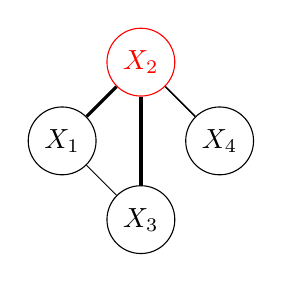
\begin{tikzpicture}
                                \node[circle, draw] (A) at (0,0) {$X_1$};
                                \node[circle, color=red, draw] (B) at (1,1) {$X_2$};
                                \node[circle, draw] (C) at (1,-1) {$X_3$};
                                \node[circle, draw] (D) at (2,0) {$X_4$};
                                \draw[line width=0.4mm] (A) -- (B);
                                \draw[line width=0.1mm] (A) -- (C);
                                \draw[line width=0.2mm] (B) -- (D);
                                \draw[line width=0.6mm] (C) -- (B);
                            \end{tikzpicture}
                        \end{column}
                        \begin{column}{0.4\textwidth}
                        % \begin{gather*}
                                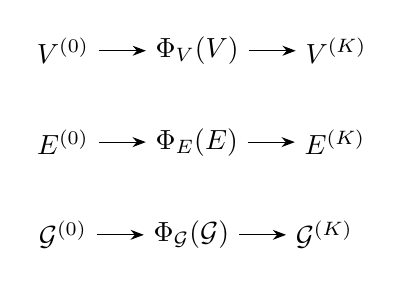
\begin{tikzpicture}[node distance=0.6cm,>=Stealth]
                                    % Nodes
                                    \node (NodeSet0) {$\NodeSet^{(0)}$};
                                    \node[right=of NodeSet0] (PhiNodeSet) {$\Phi_\NodeSet(\NodeSet)$};
                                    \node[right=of PhiNodeSet] (NodeSetIter) {$\NodeSet^{(\Iter)}$};
                                
                                    \node[below=of NodeSet0] (EdgeSet0) {$\EdgeSet^{(0)}$};
                                    \node[right=of EdgeSet0] (PhiEdgeSet) {$\Phi_\EdgeSet(\EdgeSet)$};
                                    \node[right=of PhiEdgeSet] (EdgeSetIter) {$\EdgeSet^{(\Iter)}$};
                                
                                    \node[below=of EdgeSet0] (Graph0) {$\Graph^{(0)}$};
                                    \node[right=of Graph0] (PhiGraph) {$\Phi_\Graph(\Graph)$};
                                    \node[right=of PhiGraph] (GraphIter) {$\Graph^{(\Iter)}$};
                                
                                    % Arrows
                                    \draw[->] (NodeSet0) -- (PhiNodeSet);
                                    \draw[->] (PhiNodeSet) -- (NodeSetIter);
                                
                                    \draw[->] (EdgeSet0) -- (PhiEdgeSet);
                                    \draw[->] (PhiEdgeSet) -- (EdgeSetIter);
                                
                                    \draw[->] (Graph0) -- (PhiGraph);
                                    \draw[->] (PhiGraph) -- (GraphIter);
                                \end{tikzpicture}
                        %\end{gather*}
                        \end{column}
                        \begin{column}{0.3\textwidth}
                            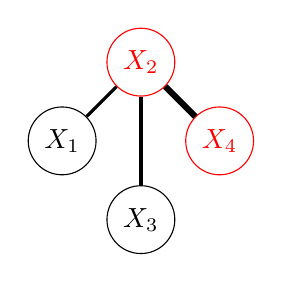
\begin{tikzpicture}
                                \node[circle, draw] (A) at (0,0) {$X_1$};
                                \node[circle, color=red, draw] (B) at (1,1) {$X_2$};
                                \node[circle, draw] (C) at (1,-1) {$X_3$};
                                \node[circle, color=red, draw] (D) at (2,0) {$X_4$};
                                \draw[line width=0.4mm] (A) -- (B);
                                %\draw[line width=0.1mm] (A) -- (C);
                                \draw[line width=0.8mm] (B) -- (D);
                                \draw[line width=0.5mm] (C) -- (B);
                            \end{tikzpicture}
                        \end{column}
                        \end{columns}

                    \end{frame}

\fi


\begin{frame}{
    General Framework\footnote{See \cite{ektefaie_multimodal_2023,gilmer_neural_2017, xu_how_2019}}
    }

    We begin with the general Message Passing Neural Networks (MPNN) structure of a GNN: 

    \vspace{4mm}
    
    \begin{algorithmic}[1]
    \State Initialize $\nrepresent^{(0)} \gets x_\node, \forall \node \in \NodeSet$ 
        \For{$\iter = 0, ..., \Iter$}:
            \For{$\node \in \Graph$}:
            \State $m_u^{(\iter+1)} \gets \text{\textcolor{blue}{Message}}(\nrepresent_\node^{(\iter)}, \nrepresent^{(\iter)}_u, \edge_{\node u}), \forall u \in \nhood_\node$
            \State $\nrepresent_{agg}^{(\iter+1)} \gets \text{\textcolor{blue}{Aggregate}}(\{m_u^{(\iter)} \mid u \in \nhood_\node\})$ 
            \State $\nrepresent^{(\iter+1)} \gets \text{\textcolor{blue}{Update}}(\nrepresent^{(\iter)}, \nrepresent_{agg}^{(\iter)})$
            \EndFor
        \EndFor
        \State $\hat{y} \gets \text{\textcolor{blue}{Transform}}(\{h^\Iter_\node | \node \in \Graph\})$ 
        \qquad{\hspace{4mm} or \textcolor{blue}{Readout$(\cdot)$}}
    \end{algorithmic}   

\end{frame}




\begin{frame}{General Framework}
Can succinctly represent the $\iter$th layer as: 
\begin{align*}
\iffalse 
    \mathbf{h}_\node^{(\iter+1)} 
    &=
    \text{Update}
    \left\{ 
    x_\node^{(\iter)}
    ,   
    \text{Aggregate}
    \left[
        \text{Message}
        \left(
        h_\node^{(\iter)}, x_u^{(\iter)}, \edge_{u,\node}^{(\iter)}
        \right)
    \right]
    \right\}
\\
\fi
    h_\node^{(\iter+1)} 
    &=
    Up
    \left\{ 
    \nrepresent_\node^{(\iter)}
    ,   
    Agg
    \left[
        Msg
        \left(
        h_\node^{(\iter)}, x_u^{(\iter)}, \edge_{u,\node}^{(\iter)}
        \right)
    \right]
    \right\}
\end{align*}

Choices of (differentiable) functions for Aggregate, Update, and Readout determine the architecture of your GNN 

\vspace{4mm}

Trained end-to-end via backpropagation for problem-specific Transform function 

\end{frame}

\begin{frame}{Aggregate \& Update}
    \begin{itemize}
        \item {\bf Aggregate$(\cdot)$} produces a representation of information from a node's neighborhood via {\bf permutation invariant} function
        \item Can include weights (edge-wise or learned)
        \item Over later iterations, this includes information from further and further distant nodes to any one target node 
        \item We then {\bf Update$(\cdot)$} our current state using this aggregated neighborhood-level information
    \end{itemize}
\end{frame}


\begin{frame}{Transform/Readout}
    \begin{itemize}
        \item {\bf Transform$(\cdot)$ } translates our learned node representations to some desired outcome 
        \begin{itemize}
            \item Regression
            \item Binary/Multi-class classification 
            \item MLP/DNN's 
        \item {\bf Readout$(\cdot)$} is common term for translating node-level output to graph-level
            \item {\it Global Pooling} - Methods applied over entire graph (e.g. averaging, fitting "regular" deep neural network, etc.)
        \end{itemize}
    \end{itemize}
\end{frame}





\begin{frame}{Graph Convolutional Network}
    \begin{itemize}
    \item Proposed in 2017 by Thomas Kipf, Max Welling \cite{kipf_semi-supervised_2017}, can consider one example of "Laplacian-based methods" \cite{gilmer_neural_2017} 
    \end{itemize}
    
        \begin{align*}
        \iffalse
            \mathbf{\nrepresent}_\node^{(\iter+1)} 
            &=
            \text{Update}
            \left( 
            x_\node^{(\iter)}
            ,   
            \text{Aggregate}
            (
                \nrepresent_\node^{(\iter)}, x_u^{(\iter)}, \edge_{u,\node}^{(\iter)}
            )
            \right)
        \\
        \fi 
            \NodeRepMat^{(\iter+1)} 
            &=
            \ReLu
            \left( 
                \mathbf{
                %D^{-1/2}
                %(\AdjMat + I)
                %D^{-1/2}
                \widetilde{\DegMat}^{-1/2}
                \widetilde{\AdjMat}
                \widetilde{\DegMat}^{-1/2}  
                \NodeRepMat^{(\iter)}
                \Theta 
                }            
            \right)
    \end{align*}
    
    \begin{itemize}
        \item Motivated by considering the graph convolution\footnote{$U$ the matrix of eigenvectors of $\LapMat$} $x \star g = UgU^Tx$ as the message passing function 
        \item Learned weight/parameter matrix $\boldsymbol\Theta$
        %\item $\mathbf{D}_{ii} = \sum_{j}\mathbf{(\AdjMat+I)_{ij}}$
        %\item Eigenvalue normalizing $\mathbf{D^{-1/2}(\AdjMat + I)D^{-1/2}}$ for computational stability
    \end{itemize}
    \end{frame}




\begin{frame}{Graph Convolutional Network}
    Intuitive "derivation": 
    \begin{align*}
        \NodeRepMat^{(\iter+1)}
        &=
        \sigma
        \left( 
            \AdjMat \NodeRepMat^{(\iter)} \Theta
        \right) 
    \\
        \NodeRepMat^{(\iter+1)}
        &=
        \sigma
        \left( 
            \DegMat^{-1}\AdjMat \NodeRepMat^{(\iter)} \Theta
        \right) 
        \qquad{\text{Normalizing by degree}}
    \\
        \NodeRepMat^{(\iter+1)}
        &=
        \sigma
        \left( 
            \DegMat^{-1/2}\AdjMat\DegMat^{-1/2} \NodeRepMat^{(\iter)} \Theta
        \right) 
        \qquad{\text{Symmetric normalization}} % "no longer simple averaging"
    \\
        \NodeRepMat^{(\iter+1)}
        &=
        \sigma
        \left( 
            \widetilde{\DegMat}^{-1/2}
            \widetilde{\AdjMat}
            \widetilde{\DegMat}^{-1/2} \NodeRepMat^{(\iter)} \Theta
        \right) 
        \qquad{\text{Adding self-loop}}
    \end{align*}
    
    where $\widetilde{\AdjMat} = \AdjMat + \Identity, \widetilde{\DegMat}_{ii} = \sum_j \widetilde{\AdjMat}_{ij}$, $\sigma$ is any activation function, $\NodeRepMat$ is simply the matrix of $\mathbf{\nrepresent}_\node$ for all nodes 
    % intuition here is normalizing by a nodes degree (left mult) and "averaging" neighborhood degree (right mult)
    % nice explainer \url{https://math.stackexchange.com/questions/3035968/interpretation-of-symmetric-normalised-graph-adjacency-matrix}
\end{frame}

\begin{frame}{Graph Convolutional Network}
    \begin{itemize}
    \item Proposed in 2017 by Thomas Kipf, Max Welling \cite{kipf_semi-supervised_2017}, can consider one example of "Laplacian-based methods" \cite{gilmer_neural_2017} 
    \end{itemize}
    
    \begin{align*}
        \iffalse
            \mathbf{\nrepresent}_\node^{(\iter+1)} 
            &=
            \text{Update}
            \left( 
            x_\node^{(\iter)}
            ,   
            \text{Aggregate}
            (
                \nrepresent_\node^{(\iter)}, x_u^{(\iter)}, \edge_{u,\node}^{(\iter)}
            )
            \right)
        \\
        \fi 
            \NodeRepMat^{(\iter+1)} 
            &=
            \underbrace{\ReLu}_{\text{Update}}
            \underbrace{
            \left( 
                \mathbf{
                %D^{-1/2}
                %(\AdjMat + I)
                %D^{-1/2}
                \widetilde{\DegMat}^{-1/2}
                \widetilde{\AdjMat}
                \widetilde{\DegMat}^{-1/2}  
                \NodeRepMat^{(\iter)}
                \Theta 
                }            
            \right)
            }_{\text{Aggregate/Message}}
    \end{align*}
    
    \begin{itemize}
        \item Motivated by considering the graph convolution\footnote{$U$ the matrix of eigenvectors of $\LapMat$} $x \star g = UgU^Tx$ as the message passing function 
        \item Learned weight/parameter matrix $\boldsymbol\Theta$
        %\item $\mathbf{D}_{ii} = \sum_{j}\mathbf{(\AdjMat+I)_{ij}}$
        %\item Eigenvalue normalizing $\mathbf{D^{-1/2}(\AdjMat + I)D^{-1/2}}$ for computational stability
    \end{itemize}
    \end{frame}





\begin{frame}{General Framework (Revisited)}
    \begin{itemize}\setlength\itemsep{8mm}
        \item {\bf Input} 
            \begin{itemize}
                \item Node conceptualization
                \item Node embeddings
            \end{itemize}
        \item {\bf Architecture}
            \begin{itemize}
                \item Message Passing Neural Network (MPNN) 
                \item $\NodeRepMat^{(\iter+1)} 
                =
                \ReLu
                \left( 
                    \mathbf{
                    %D^{-1/2}
                    %(\AdjMat + I)
                    %D^{-1/2}
                    \widetilde{\DegMat}^{-1/2}
                    \widetilde{\AdjMat}
                    \widetilde{\DegMat}^{-1/2}  
                    \NodeRepMat^{(\iter)}
                    \Theta 
                    }            
                \right)$
            \end{itemize}
        \item {\bf Output}
            \begin{itemize}
                \item Target output (Readout, Transform functions)
                \item Loss function
            \end{itemize}
\end{itemize}
\end{frame}




\section{Applications and Extensions}
\OutlineRedux



\subsection{Structure-Based Drug Design (SBDD)}

\begin{frame}{}
    \textbf{\Large Proteins and Structure-Based Drug Design (SBDD)} \\ 
    \vspace{5mm}
    Geometric Deep Learning for Structure-Based Drug Design: A Survey
(2023) \\ 
Zaixi Zhang, Jiaxian Yan, Qi Liu, Enhong Chen, and Marinka Zitnik
\cite{zhang_systematic_2023}
\end{frame}



\begin{frame}{Structure-Based Drug Design (SBDD)}
    \begin{itemize}
        \item SBDD aims to improve drug-discovery by understanding 3D protein structures and predicting drug efficacy/behavior % docking, conformations, etc. summarize as useful to understand behavior of drug based on target protein structure 
        \item Can dichotomize tasks categorized as \textit{predictive} or \textit{generative}
        \item Problems of note for GNN's include predictive tasks 
        \begin{itemize}
            \item \textbf{binding site prediction} 
            \item \textbf{binding affinity prediction}
        \end{itemize}
        \item Other characteristics are important for drug design and protein-ligand interactions but without current GNN methods to my knowledge 
        \begin{itemize}
            \item Binding pose 
            \item Ligand generation 
            \item Linker design 
        \end{itemize}
%        \item Protein Databank (PDB), PDBBind, Dockground, CSAR-HiQ are existing data sets used to train most GNN's in these contexts 
    \end{itemize}
\end{frame}

\begin{frame}{Output}
    \begin{itemize}
        \item {\bf Binding site prediction} is binary categorization at the (surface) amino acid level 
        \item {\bf Binding affinity prediction} is a continuous measure of protein-ligand interaction strength 
    \end{itemize}

    \vspace{4mm}

    \begin{columns}
        \begin{column}{0.5\textwidth}
            \includegraphics[width=\textwidth]{Zhang_2023_BindingSite.png}
        \end{column}
        \begin{column}{0.5\textwidth}
            \includegraphics[width=\textwidth]{Zhang_2023_BindingAffinity.png}
        \end{column}
    \end{columns}
    \centering{\small Images from Fig. 1 of Zhang (2023) \cite{zhang_systematic_2023}}
\end{frame}

\iffalse 
            \begin{frame}{Input}
                \begin{columns}
                \begin{column}{0.7\textwidth}
                \begin{itemize}\setlength\itemsep{6mm}
                    \color{red}
                    \item Nodes are radial patches (i.e. points)
                    \item Focus on complications of 3D geometry 
                    \vspace{8mm}
                    \begin{minipage}{\textwidth}
                    \item Invariant, necessary as previously stated ("coordinate system robust")
                    \item Equivariant, less strict than invariant, some transformations should generate different output (see protein conformations for drug-ligand interaction) 
                    \end{minipage}
                \end{itemize}
                \end{column}

                \begin{column}{0.3\textwidth}
                    \vspace*{-12mm}
                    %\begin{figure}
                        \begin{flushright}
                        \includegraphics[width=\textwidth]{Gainza_2020_ProteinNodesRadii.png}  \\ 
                        Fig 1a. Gainza (2020) \cite{gainza_deciphering_2020}
                        \end{flushright}
                    %\end{figure}    
                \end{column}
            \end{columns}
            \end{frame}
\fi 





\begin{frame}{Input}
    \begin{figure}
        \centering 
        \includegraphics[scale=0.55]{Isert_2023_ModelsSBDD.png}
    \end{figure}
    Figure from Isert (2023) \cite{isert_structure-based_2023}
\end{frame}

\begin{frame}{CNN Input}
    \begin{itemize}
        \item Nodes and edges defined by radial patches about a discretization of the protein surface 
    \end{itemize}

    \begin{figure}
        \centering 
        \includegraphics[scale=0.4]{Isert_2023_ModelsSBDD_VoxelMesh.png}
%    \end{figure}
%
%    \begin{figure}
%        \centering
        \includegraphics[scale=0.5]{Gainza_2020_ProteinNodesRadii.png}  \\ 
        Left: Fig 2(ab) from Isert (2023); Right: Fig 1a. Gainza (2020) \cite{isert_structure-based_2023, gainza_deciphering_2020}
    \end{figure}
\end{frame}



\begin{frame}{GNN Input}
    \begin{columns}
        \begin{column}{0.65\textwidth}
            \begin{itemize}\setlength\itemsep{6mm}
                \item Nodes $\node$ include typical feature embeddings $\nrepresent$ and 3-dimensional coordinate data $\mathbf\node$
                \item Nodes are primarily conceptualized at the {\bf amino acid} (also {\bf residue}) level
                    %\item Can also consider the atomic sub-structure
                \item Maintain invariance for translations, rotations but not necessarily reflections 
            \end{itemize}            
        \end{column}
        \begin{column}{0.35\textwidth}
            \begin{figure}
                \centering 
                \includegraphics[scale=0.55]{Isert_2023_ModelsSBDD_3DGraph.png}
            \caption{Figure 1c from Isert (2023) \cite{isert_structure-based_2023}}
        \end{figure}
                    
        \end{column}
    \end{columns}
\end{frame}


\begin{frame}{Architecture}
Consider some transformations $T, T'$ (e.g. reflection, rotation, etc.) within the same symmetry group: \newline 
\vspace{3mm} 
\\ 

Invariance: $f(T(x)) = T'(f(x)) = f(x)$
\\
\vspace{6mm}

Equivariance: 
$\forall  T, \  \exists T': f(T(x)) = T'(f(x))$

\end{frame}

\begin{frame}{Architecture(s)}
Forgoing the iteration supercripts, one message pass can be represented as such: 
    \begin{align*}
        m_{ij}
        &=
        \textcolor{blue}{Msg_m}(\mathbf{\node_i}, \mathbf{\node_j}, \nrepresent_i, \nrepresent_j, \edge_{ij}) 
    \\ 
        \mathbf{m}_{ij}
        &=
        Msg_{\mathbf{m}}
        (\mathbf{\node_i}, \mathbf{\node_j}, \nrepresent_i, \nrepresent_j, \edge_{ij})
    \\
        \nrepresent_i'
        &=
        \textcolor{blue}{Update_\nrepresent}
        \left[
            \nrepresent_i
            , 
            Agg_h
            (
                \{m_{ij}\}_{j \in \nhood(\node_i)}
            )
        \right]     
    \\
        \mathbf{\node_i'}
        &=
        Update_{\mathbf\node}
        \left[
            \mathbf{\node}_i
            , 
            Agg_\mathbf{\node}
            \left( 
                \{\mathbf{m}_{ij}\}_{j \in \nhood(\node_i)}
            \right)
        \right]
    \end{align*}

    where \textcolor{blue}{$Msg_m, Update_h$} are geometrically {\bf invariant}, scalar functions and $Msg_{\mathbf{m}}, Update_{\mathbf\node}$ are geometrically {\bf equivariant}, vector functions \newline 
    Here $\mathbf\node \in \mathbb{R}^3$ are 3-D coordinates (e.g. atom or amino acid location)\\
\end{frame}


\iffalse 
        \begin{frame}{Architecture(s)}
            May also consider the proposed Equivariant Graphical Neural Network (EGNN) from Satorras (2021) \cite{satorras_en_2022}. Again, let $\mathbf{\node}_i$ represent a node's coordinate embeddings: 
                \begin{align*}
                    m_{ij}
                    &=
                    Msg_m(\nrepresent_i, \nrepresent_j, ||\mathbf{\node}_i^{(\iter)}-\mathbf{\node}_j^{(\iter)}||^2, \edge_{ij}) 
                \\ 
                    \mathbf{\node}_i^{(\iter+1)}
                    &=
                    \mathbf{\node}_i^{(\iter)}
                    +
                    C
                    \sum_{j\neq 1}
                    \left(
                    \mathbf{\node}_i^{(\iter)}
                    -
                    \mathbf{\node}_j^{(\iter)}
                    \right) 
                    Agg_\node(m_{ij})
                \\
                    m_i 
                    &= 
                    Agg(m_{ij})
                    =
                    \sum_{j\neq i} m_{ij}
                \\
                    \nrepresent^{(\iter+1)}
                    &=
                    Update(\nrepresent^{(\iter+1)}, m_i)
                \end{align*}
            
        \end{frame}
\fi 
    
\begin{frame}{NodeCoder}
    \begin{figure}
        \centering 
        \includegraphics[scale=0.3]{Fig1_NodeCoder.png}
        \caption{Subst of Fig. 1 from Abdollahi (2023) NodeCoder \cite{abdollahi_nodecoder_2023}}
    \end{figure}

    \begin{itemize}
        \item Nodes are residues with atomic property (and other) embeddings
        \item With a given layer updated using a slight adaptation of GCN: 
    \end{itemize}
    \begin{align*}
        \NodeRepMat^{(\iter+1)} 
        &=
        \text{ELu}
        \left( 
            \mathbf{
            %D^{-1/2}
            %(\AdjMat + I)
            %D^{-1/2}
            \widetilde{\DegMat}^{-1/2}
            \widetilde{\AdjMat}
            \widetilde{\DegMat}^{-1/2}  
            \NodeRepMat^{(\iter)}
            \Theta 
            }            
        \right)
    \\
        \NodeRepMat^{(\Iter)} 
        &=
        LogSoftMax
        \left\{
        \widetilde{\DegMat}^{-1/2}
        \widetilde{\AdjMat}
        \widetilde{\DegMat}^{-1/2}  
        \text{ELu}
        \left( 
            \mathbf{
            %D^{-1/2}
            %(\AdjMat + I)
            %D^{-1/2}
            \widetilde{\DegMat}^{-1/2}
            \widetilde{\AdjMat}
            \widetilde{\DegMat}^{-1/2}  
            \NodeRepMat^{(\iter)}
            \Theta 
            }            
        \right)
        \Theta_t
        \right\}
    \end{align*}
\end{frame}




\begin{frame}{PIGNet}
    \begin{figure}
        \centering 
        \includegraphics[scale=0.6]{Zhang_Fig8_Binding.png}
        \caption{Fig 8. from Zhang (2023) describing PIGNet architecture \cite{moon_pignet_2022, zhang_systematic_2023}}
    \end{figure}
\end{frame}


\begin{frame}{ScanNet}
    \begin{figure}
        \centering 
        \includegraphics[scale=0.35]{ScanNet_Pooling.png}
        \caption{Fig 1. from Tubiana (2021) \cite{tubiana_scannet_2022}}
    \end{figure}
\end{frame}

\begin{frame}{SBDD Summary}
    \begin{itemize}\setlength\itemsep{6mm}
        \item Geometric Deep Learning is used to predict protein properties (in addition to drug-ligand interactions)
        \item Conceptualize nodes as residues 
        \begin{itemize}
            \item Can also fix graph with atomic nodes, fit GNN (or other methdo) to input atomic graph, and pool at the residue level  
        \end{itemize}
        \item Adapt our architecture to account for desired geometric invariance and equivariance 
        \item Zhang (2023) \cite{zhang_systematic_2023} review compiles these and more complex architectures
        \begin{itemize}
            \item Transformers 
            \item Variational Autoencoders 
            \item Methods for generative GDL tasks 
        \end{itemize}
    \end{itemize}
\end{frame}



\subsection{Multimodal Graph Learning (MGL)}


\begin{frame}{}
    \textbf{\Large Multimodal Graph Learning (MGL)}  \\
    \vspace{5mm}
    Multimodal learning with graphs (2023) \\ Yasha Ektefaie, George Dasoulas, Ayush Noori, Maha Farhat, and Marinka Zitnik
\end{frame}


\begin{frame}{Motivation}
    \begin{figure}
        \centering
        \includegraphics[scale=0.25]{Multimodal_Concep.png}
        \caption{Fig. 3 from Li (2022) \cite{li_graph_2022}}
    \end{figure}
\end{frame}




\begin{frame}{Multimodal Graph Learning (MGL)}
\begin{itemize}\setlength\itemsep{6mm}
    \item Ektefaie (2023) {\it Multimodal learning with graphs} \cite{ektefaie_multimodal_2023}
    \item Topology is complicated by multimodality of input data 
    \begin{itemize}
        \item Modal collapse \cite{javaloy_mitigating_2022}
        \item Differential data availability 
    \end{itemize}
\end{itemize}    
\vspace{3mm}
    \begin{columns}[T]
        \begin{column}{0.5\textwidth}
            Clinical Data
            \begin{itemize}        
                \item Clinical text  
                \item -omics data 
                \item Laboratory measurements 
                \item Clinical imaging
            \end{itemize}
            \end{column}
        \begin{column}{0.5\textwidth}
            Protein Structures
            \begin{itemize}        
                \item 1$^\circ$ AA Sequence
                \item 2$^\circ$ Helix interactions
                \item 3$^\circ$ Folding, bridges 
            \end{itemize}
        \end{column}
%        \begin{column}{0.3\textwidth}
%            Text Data
%            \begin{itemize}        
%                \item 
%            \end{itemize}
%        \end{column}
    \end{columns}
\end{frame}

\begin{frame}{Aggregation}
    \begin{figure}
        \centering 
        \includegraphics[scale=0.6]{Modal_Agg_Fig2.png}
        \caption{Subet of Fig. 2 from Ektefaie (2023) \cite{ektefaie_multimodal_2023}}
    \end{figure}
\end{frame}


\begin{frame}{Framework}
    Authors propose a four component "blueprint"
    \begin{enumerate}
    \item Identifying entitites (i.e. modalities)
    \item Uncovering topology 
    \begin{itemize}
        \item {\it A priori}
        \item Adaptively learned
    \end{itemize}
    \item Propagating information 
    \item Mixing representation 
    \end{enumerate}
\end{frame}


\begin{frame}{Framework}
    Authors propose a four component "blueprint"
    \begin{enumerate}
    \item Identifying entitites (i.e. modalities)
    \item Uncovering topology 
    \item Propagating information
    \item Mixing representation
    \end{enumerate}
    \begin{tikzpicture}[overlay,remember picture]
        \draw[decorate,decoration={calligraphic brace, amplitude=4pt},line width=1.2pt]
        (6.7,2.6) -- (6.7,1.7) node[midway, right=6pt, xshift=-2pt, text=black] {\footnotesize Structure Learning};
    \end{tikzpicture}

    \begin{tikzpicture}[overlay,remember picture]
        \draw[decorate,decoration={calligraphic brace, amplitude=4pt},line width=1.2pt]
        (5.2,1.8) -- (5.2,0.95) node[midway, right=6pt, xshift=-2pt, text=black] {\footnotesize Learning On-Structure Phase};
    \end{tikzpicture}
\end{frame}

\begin{frame}{Structure Learning}
    \begin{columns}[T]
    \begin{column}{0.5\textwidth}
        %\vspace{12mm}
        \begin{itemize}
            \item Consider modalities as {\it entities} (colored nodes)
            \begin{itemize}
                \item Clinical text/narrative data 
                \item Laboratory/Physiological measurements 
                \item Image/Video data 
                \item Patient reported measurements/symptoms
                \item etc. 
            \end{itemize}
            \item Use known modalities to \textbf{identify} nodes
            \item \textbf{Connect} nodes to generate graph structure (learned or provided \textit{a priori} knowledge)
        \end{itemize}      
    \end{column}
    \begin{column}{0.5\textwidth}
        \begin{figure}
            \includegraphics[scale=0.4]{Ektefaie_StructureLearning.png}
            \caption{Subset of Fig 2c \cite{ektefaie_multimodal_2023}}
        \end{figure}    
    \end{column}
\end{columns}
\end{frame}



\begin{frame}{Learning on Structure}
    \begin{columns}[T]
    \begin{column}{0.5\textwidth}
        %\vspace{12mm}
        \begin{itemize}
            \item Can construct one or more adjacency measures $\mathbf{A}$ 
            \item Message propagate across edges outlined in Structure Learning 
            \item Combine representations 
            \begin{itemize}
                \item Summation 
                \item Averaging 
                \item Neighborhood-specific aggregation
            \end{itemize}
        \end{itemize}      
    \end{column}
    \begin{column}{0.5\textwidth}
        \begin{figure}
            \includegraphics[scale=0.4]{Ektefaie_OnStructure.png}
            \caption{Subset of Fig 2c \cite{ektefaie_multimodal_2023}}
        \end{figure}    
    \end{column}
\end{columns}
\end{frame}

\begin{frame}{}
    \begin{figure}
        \centering 
        \includegraphics[scale=0.4]{MGL_MethodsTable.png}
        \caption{Supp. Table 2 from Ektefaie (2023) \cite{ektefaie_multimodal_2023}}
    \end{figure}
\end{frame}


\begin{frame}{TextGCN}
    \begin{itemize}
        \item Graph-building by word co-occurrence(\textit{uncovering toplogy}) 
        \item $Z = SoftMax(
            \widetilde{\DegMat}^{-1/2}
            \widetilde{\AdjMat}
            \widetilde{\DegMat}^{-1/2}  
            \ReLu(\widetilde{\DegMat}^{-1/2}
            \widetilde{\AdjMat}
            \widetilde{\DegMat}^{-1/2}  
            \NodeRepMat^{(\iter)}\Theta)\Theta^*)$
    \end{itemize}
    \begin{figure}
        \centering 
        \includegraphics[scale=0.4]{TextGCN_Yao_Fig2.png}
        \caption{Figure 1 from Yao (2018) \cite{yao_graph_2018}}
    \end{figure}
\end{frame}


\begin{frame}{Zheng (2022) Multi-modal Graph Learning for Disease Prediction }
    \begin{figure}
        \centering 
        \includegraphics[scale=0.4]{Zheng_2022_MGL_Patients_Arch.png}
        \caption{Fig. 2. From Zheng (2022) \cite{zheng_multi-modal_2022}}
    \end{figure}
\end{frame}




\begin{frame}{Summary of Multimodal Graph Learning}
    \begin{itemize}\setlength\itemsep{6mm}
        \item Accounting for intermodal information (currently) arises in graph-learning stages 
        \item Quite comprehensive framework, includes some early GDL/CNN papers and methods 
        \begin{itemize}
            \item MaSIF CNN model
            \item Graph Attention Networks 
        \end{itemize} 
    \end{itemize}
\end{frame}


\subsection{TxGNN}

\begin{frame}{}
    \textbf{\Large TxGNN: Geometric Deep Learning and "Human-Centered AI"}  \\
    \vspace{5mm}
    Zero-shot prediction of therapeutic use with geometric deep learning and clinician centered design (2023) \\ 
    Huang, Chandak, Wang, Havaldar, Vaid, Leskovec, Nadkarni, Glicksberg, Gehlenborg, Zitnik
\end{frame}

\begin{frame}{Motivation}
    \begin{itemize}\setlength\itemsep{6mm}
        \item TxGNN trained to predict therapeutic agents for "neglected" diseases 
        \item "Zero-shot prediction" - disease with few or no understood indications 
        \item Formally stated, we want to predict if drug $j$ is indicated or contraindicated for disease $i$
    \end{itemize}
\end{frame}


\begin{frame}{Input}
    \begin{figure}
        \centering 
        \includegraphics{txGNN_KG.png}
        \caption{Fig 1A from Huang (2023) \cite{huang_zero-shot_2023}}
    \end{figure}
\end{frame}



\begin{frame}{Harmonization and PrimeKG}
%    \begin{figure}
%        \centering 
%        \includegraphics[scale=0.4]{Huang_NodeTypes.png}
%        \caption{Table 3 from Huang (2023) \cite{huang_zero-shot_2023}}
%    \end{figure}
    \begin{itemize}
        \item Chandak (2023) \textit{"Building a knowledge graph to enable precision medicine"} paper provides framework on KG harmonization \cite{chandak_building_2023}
        \item Define common ontologies and construct an aggregated KG from heterogeneous sources 
        \begin{itemize}
            \item "drug", "disease", "anatomy", "pathway", "biological process", "molecular function", "gene/protein", "effect/phenotype", "exposure"
        \end{itemize}
    \end{itemize}

    \begin{figure}
        \centering 
        \includegraphics[scale=0.4]{Chandak_KG_Arch.png}
        \caption{Fig. 2a from Chandak (2023) \cite{chandak_building_2023}\footnote{This does not reflect the specific data sources in TxGNN, although there is some overlap, just a general data harmonization outline}}
    \end{figure}
\end{frame}


\begin{frame}{Input}
    Represent our KG $\Graph = (\NodeSet, \EdgeSet, \RelationSet), \edge_{ij} = (\node_i, \relation, \node_j)$ and our usual node-embedding notation $\nrepresent_i$
    \begin{figure}
        \centering 
        \includegraphics[scale=0.85]{txGNN_KG.png}
        \caption{Fig 1A from Huang (2023) \cite{huang_zero-shot_2023}}
    \end{figure}
\end{frame}



\begin{frame}{Architecture}
    \begin{figure}
        \centering
        \includegraphics[scale=0.4]{TxGNN_Arch.png}
        \caption{Fig. 1b from Huang (2023) \cite{huang_zero-shot_2023}}
    \end{figure}
\end{frame}

\begin{frame}{Architecture}
    \begin{enumerate}
        \item A heterogeneous graph neural network-based encoder to obtain biologically meaningful network representation for each biomedical entity
        \item A disease similarity-based metric learning decoder to leverage auxiliary information to enrich the representation of diseases that lack molecular characterization
        \item An all-relation stochastic pre-training followed by a drug-disease centric full-graph fine-tuning strategy
        \item A graph explainability module to retain a sparse set of edges that are crucial for prediction as a post-training step
      \end{enumerate}
\end{frame}

\begin{frame}{Architecture}
    \begin{enumerate}
        \item $\relation-$MPNN
        \item Disease similarly quantification (and gatekeeping)
        \item Pre-train on KG mini-batches; Fine-tune on drug-disease pairs 
        \item Interpretability 
      \end{enumerate}
\end{frame}

\begin{frame}{Heterogenous graph neural network encoder}
    Here, let $\nhood_\relation$ be the neighborhood only for edges of relation type $r$
    \begin{align*}
        Message:
        &
        m_{\relation,i} 
        = 
        \Theta_{\relation,M}\nrepresent_i
        \\
        Aggregate:
        &
        \widetilde{m_{\relation,i}} 
        = 
        |\nhood_{\relation (i)}|^{(-1)}
        \sum_{j \in \nhood_{\relation (i)}}
        m_{\relation,j}
        \\
        Update:
        &
        h_i 
        \leftarrow 
        h_i + \sum_{\relation \in \RelationSet}
        \widetilde{m_{\relation,i}} 
        \\
        \\
        &p_{i,j,r} 
        =
        expit(\sum \nrepresent_i \cdot w_r \cdot \nrepresent_j)
        \\
        &
        \Loss 
        =
        \sum_{(i,r,j)}
%        \sum_{(i,r,j) \in D_+ \cup D_-}
        y_{i,r,j} * \log(p_{i,r,j})
        +
        (1-y_{i,r,j}) * \log(1-p_{i,r,j})
    \end{align*}
\end{frame}

\begin{frame}{Disease Similarity}
    \begin{itemize}\setlength\itemsep{4mm}
        \item Recall TxGNN's goal is zero-shot for poorly-understood diseases (i.e. likely sparsely connected) 
        \item Rather than update these embeddings, identify most similar and well-understood diseases to utilize KG information 
        \begin{itemize}
            \item Protein structure similarity 
            \item Similar phenotype or exposure 
        \end{itemize}
        \item Supply a "gating mechanism" to induce similarity updating of poorly-understood diseases while discouraging updating well-connected/known diseases 
    \end{itemize}
\end{frame}


\iffalse 
            \begin{frame}{Architecture}
                Loss function: 
                \begin{gather*}
                    \Loss 
                    =
                    \sum_{(i,r,j) \in D_+ \cup D_-}
                    y_{i,r,j} * \log(p_{i,r,j})
                    +
                    (1-y_{i,r,j}) * \log(1-p_{i,r,j})
                \end{gather*}
            Train/Test Split:
                \begin{itemize}
                    \item Test-train split by \textit{a priori} defined disease groups 
                    \item Random test-train split $\rightarrow$ all drug-disease connections moved to test set among test disease sets 
                \end{itemize}
            \end{frame}
\fi 

\begin{frame}{Pre-training/Fine-tuning}
    \begin{itemize}\setlength\itemsep{4mm}
        \item Desire for PT/FT is two-fold: computation and scope 
        \item Pre-train on random mini-batches 
        \item Use pre-trained encoder weights (with exception of $w_r$) for fine-tuning on drug-disease pairs 
    \end{itemize}
\end{frame}



\begin{frame}{Architecture (Revisited)}
    \begin{figure}
        \centering
        \includegraphics[scale=0.4]{TxGNN_Arch.png}
        \caption{Fig. 1b from Huang (2023) \cite{huang_zero-shot_2023}}
    \end{figure}
\end{frame}

\begin{frame}{Explainability}
    \begin{itemize}
        \item Account for lack of interpretability of model parameters by identifying sparse edge sets for relevant predictions 
        \item Calculate indicator for edge inclusion $z^{(\iter)} = \mathbf{1}_{[\mathbb{R}>0.5]}
        \left( 
            \text{sigmoid}
            \left( 
                W_{g,r}^{(\iter)}(m_{r,i}^{(\iter)}||m_{r,j}^{(\iter)})
            \right)
        \right)$
        \item Update message $\hat{m}_{ir}^{(\iter)} = z_{ijr}^{(\iter)} \cdot m_{i,r}^{(\iter)} + (1-z_{i,j,r}^{(\iter)})\cdot \mathbf{b}_r^{(\iter)}$ for learnable baseline vector $\mathbf{b}_r$
        \item Train with loss function: \\ 
\end{itemize}
\[
    \max_\lambda \min_{\mathbf{W}_g}  
    \sum_{k=1}^L \sum_{(i,j,r) \in D_{+} \cup D_{-}} 
    \Ind_{[R \neq 0]}z^{(k)}_{i,j,r} 
    + 
    \lambda \left( \lVert \hat{p}_{i,j,r} - p_{i,j,r} \rVert^2 - \beta\right) 
    \]

\end{frame}


\begin{frame}{TxGNN}
    \begin{itemize}
        \item Leverage heterogeneous KG data to predict therapies for poorly understood (read: sparsely KG connected) diseases 
        \item Using large, heterogeneous KG data combined with understandings of disease similarity elucidate better understandings of rare diseases or expand use of orphan drugs 
        \item Requires a non-trivial data harmonization effort as well as a PT/FT method for computational feasibility 
        \item Authors offer an explainability analysis by identifying sparse edge sets with "faithful predictions"
    \end{itemize}
\end{frame}


\section*{Conclusion}

\begin{frame}{}
    \bf{\LARGE Conclusion}    
\end{frame}



\begin{frame}[allowframebreaks]{References}
    \begin{itemize}
    \item Some diagrams generated in conjunction with ChatGPT 3.5
    \end{itemize}
    \printbibliography 
\end{frame}


%%%%%%%%%%%%%%%%%%%%%%%%%%
%%%%%%%%%%%%%%%%%%%%%%%%%%
% Appendix 
%%%%%%%%%%%%%%%%%%%%%%%%%%
%%%%%%%%%%%%%%%%%%%%%%%%%%

\section*{Appendix}

\begin{frame}{}
\bf{\LARGE Appendix Slides}    
\end{frame}



\begin{frame}{Structure-Induced Pre-Training (1/2)}
    \begin{itemize}
        \item Consider a pre-training (PT)/fine-tuning (FT) problem 
        \item We pre-train $f_\theta:\mathcal{X}\rightarrow\mathcal{Z}$ on some PT data $\mathbf{X}_{PT} \in \mathcal{X}$ and loss function $\Loss_{PT}$
        \item Use the encoded $f(\mathbf{X}_{PT}) \in \mathcal{Z}$ on some downstream, FT tasks 
        \begin{itemize}
            \item Protein folding category, stability, amino acid properties 
            \item Text sentiment 
        \end{itemize}
        \item Applied in langauge models, protein behavior prediction 
    \end{itemize}
\end{frame}

\begin{frame}{Structure-Induced Pre-Training (2/2)}
    \begin{itemize}
        \item In addition to $\mathbf{X}_{PT}$, we also have underlying structure $\Graph_{PT}$
        \item Our PT encoder $f_\theta$ must only take $\mathbf{X}_{PT}$ as input to allow transferability to FT tasks 
        \item Decompose loss function as PT objective $\Loss_{Obj}$ and structure-inducing $\Loss_\Graph$:
    \end{itemize}

    \begin{gather*}
        \Loss_{PT}
        =
        (1-\lambda)\Loss_{Obj}
        +
        \lambda \Loss_{\Graph}
    \end{gather*}
\end{frame}


\begin{frame}{Implementations}
    \begin{itemize}
        \item \href{https://pytorch-geometric.readthedocs.io/en/latest/}{PyTorch Geometric} with directed extension \href{https://github.com/SherylHYX/pytorch_geometric_signed_directed}{PyTorch Geometric Signed Directed}
        \item \href{https://github.com/tensorflow/gnn}{TensorFlow GNN} \cite{ferludin_tf-gnn_2023}
        \item \href{https://carlolucibello.github.io/GraphNeuralNetworks.jl/dev/}{GraphNeuralNetworks.jl}
        \item \href{https://graphneural.network/}{Spektral}, Keras-based Pythhon package 
        \item Limited but some implementation in R 
        \begin{itemize}
            \item \href{https://cran.r-project.org/web/packages/scapGNN/vignettes/vignette.html}{scapGNN}, package GNN implementation but specific/narrow for single-cell -omics data 
        \end{itemize}
    \end{itemize}
\end{frame}


\begin{frame}{Abbreviated History}
    \begin{itemize}
        \item Graph Neural Network first(?) coined in Gori (2005) \cite{gori_new_2005} and subqeuently in Scarselli (2009) {\it The Graph Neural Network Model} \cite{scarselli_graph_2009}
        \item Graph Convolutional Network by Kipf (2017) \cite{kipf_semi-supervised_2017} but with similar convolutional message-passing algorithms (within GNN's) proposed in at least 2015 \cite{duvenaud_convolutional_2015}
        \item Message passing GNN proposed in Gilmer (2017), applications in molecular chemistry \cite{gilmer_neural_2017} 
    \end{itemize}
\end{frame}

\begin{frame}[allowframebreaks]{Additional Applications, Interesting Papers}
    \begin{itemize}
        \item Applications in travel time prediction, 2021 (\url{https://arxiv.org/pdf/2108.11482.pdf})
        \item Someone has compiled graph-/GNN-relevant talks for NeurIPS 2023 at \url{https://github.com/XiaoxinHe/neurips2023_learning_on_graphs}
    \end{itemize}
\end{frame}

\iffalse 
\begin{frame}{DiffPool}
    Figure 1 from Ying (2018) {\it Hierarchical Graph Representation Learning with Differentiable Pooling} \cite{ying_hierarchical_2018}
    \begin{figure}
        \centering 
        \includegraphics[scale=0.45]{DIFFPOOL_RexYing.png}
    \end{figure}
\end{frame}
\fi 

\begin{frame}{NodeCoder Embeddings}
    \begin{figure}
        \centering 
        \includegraphics[scale=0.3]{NodeCoder_S2_Embeddings.png}
        \caption{From Table S2 in Abdollahi (2023) \cite{abdollahi_nodecoder_2023}}
    \end{figure}
\end{frame}

\begin{frame}{KG AI Models}
    Full figure from McDermott et al. \cite{mcdermott_structure-inducing_2023}, cropped and presented in Introduction:
    \begin{figure}
        \centering
        \includegraphics[scale=0.13]{Junwei_KG_Models_Infograph.png}
    \end{figure}
\end{frame}

\begin{frame}{Protein Data Bank File}
    \begin{figure}
        \centering
        \includegraphics[scale=0.37]{PDB_File_Ex.png}
        \caption{Example PDB file structure/protein information. Taken directly from Wikipedia: \url{https://en.wikipedia.org/wiki/Protein_Data_Bank_(file_format)}
        }
    \end{figure}
\end{frame}
\end{document}